





\section{Can Fine-Tuning Close the \textbf{DENSEWORLD} Gap?}
\label{sec:vjepa_adaptation_baselines}

Before introducing FactorJEPA, we ask whether conventional adaptation can recover the predictive structure required by DENSEWORLD without reorganizing the JEPA predictor. We evaluate three complementary strategies: \textbf{LoRA}~\cite{hu2022lora}, \textbf{DoRA}~\cite{liu2024dora}, and \textbf{Auto-RGN}~\cite{lee2023surgical}. All use the same raw clips, optimization steps, optimizer, masking policy, and evaluation protocol; only the parameter-update mechanism changes.

Let $x$ denote a video clip; $M_c$ and $M_t$ the context and target masks; $f_\theta$ the online encoder; $\bar f_{\bar\theta}$ the momentum target encoder; and $g_\phi$ the predictor. All baselines retain the executed V-JEPA objective:
\[
\mathcal{L}_{\mathrm{JEPA}}
=
\mathbb{E}_{x}
\left[
\left\|
g_\phi\!\left(f_\theta(M_c\odot x),M_t\right)
-
\operatorname{sg}\!\left(
\bar f_{\bar\theta}(M_t\odot x)
\right)
\right\|_2^2
\right],
\]
where $\operatorname{sg}$ denotes stop-gradient. This data- and step-matched protocol isolates adaptation capacity without introducing a different prediction target or training signal.

\begin{table}[ht!]
\centering
\caption{
\textbf{Protocol-matched V-JEPA adaptation baselines.}
All methods retain the JEPA objective and train on the same raw clips; only the adaptation mechanism changes.
}
\label{tab:vjepa_adaptation_baselines}
\scriptsize
\setlength{\tabcolsep}{3pt}
\renewcommand{\arraystretch}{1.08}
\begin{tabular}{
    p{0.18\columnwidth}
    p{0.40\columnwidth}
    p{0.33\columnwidth}
}
\toprule
\textbf{Method} & \textbf{Adaptation mechanism} & \textbf{Question tested} \\
\midrule

\textbf{LoRA}~\cite{hu2022lora}
&
Adds low-rank updates,
$\Delta W=(\alpha/r)BA$, to selected frozen projections.
&
Is parameter-efficient low-rank adaptation sufficient?
\\
\midrule

\textbf{DoRA}~\cite{liu2024dora}
&
Separates weight magnitude from direction and applies low-rank updates to the directional component.
&
Does weight decomposition recover structure missed by LoRA?
\\
\midrule

\textbf{Auto-RGN}~\cite{lee2023surgical}
&
Selects transformer blocks using their relative gradient norms and updates only the selected subset.
&
Can gradient-guided selection localize the required adaptation?
\\

\bottomrule
\end{tabular}
\end{table}


For LoRA, an adapted weight matrix is
\[
W' = W_0 + \frac{\alpha}{r}BA,
\qquad
B\in\mathbb{R}^{d_{\mathrm{out}}\times r},
\quad
A\in\mathbb{R}^{r\times d_{\mathrm{in}}},
\]
where $r\ll\min(d_{\mathrm{in}},d_{\mathrm{out}})$. DoRA further separates the magnitude and direction of each weight vector:
\[
W'
=
m\odot
\frac{W_0+\Delta W}
{\left\|W_0+\Delta W\right\|},
\qquad
\Delta W=\frac{\alpha}{r}BA,
\]
allowing directional adaptation without coupling it to weight magnitude.

Following the relative-gradient-norm criterion of \citet{lee2023surgical}, our blockwise Auto-RGN implementation scores transformer block $\ell$ as
\[
s_\ell
=
\frac{
\left\|
\nabla_{\theta_\ell}\mathcal{L}_{\mathrm{JEPA}}
\right\|_2
}{
\left\|\theta_\ell\right\|_2+\epsilon
},
\qquad
\mathcal{S}_K
=
\operatorname{TopK}_{\ell}(s_\ell),
\]
and updates only $\{\theta_\ell:\ell\in\mathcal{S}_K\}$. Normalization by parameter magnitude prevents larger blocks from being favored solely because of scale. LoRA and DoRA target the same projection families, while Auto-RGN receives a matched trainable-parameter budget. Ranks, scaling coefficients, selected projections, block budgets, trainable parameter counts, and measured GPU-hours are reported in Appendix~\ref{app:adaptation_details}.




















































\begin{figure*}[ht!]
    \centering

    \begin{minipage}[t]{0.48\textwidth}
        \centering
        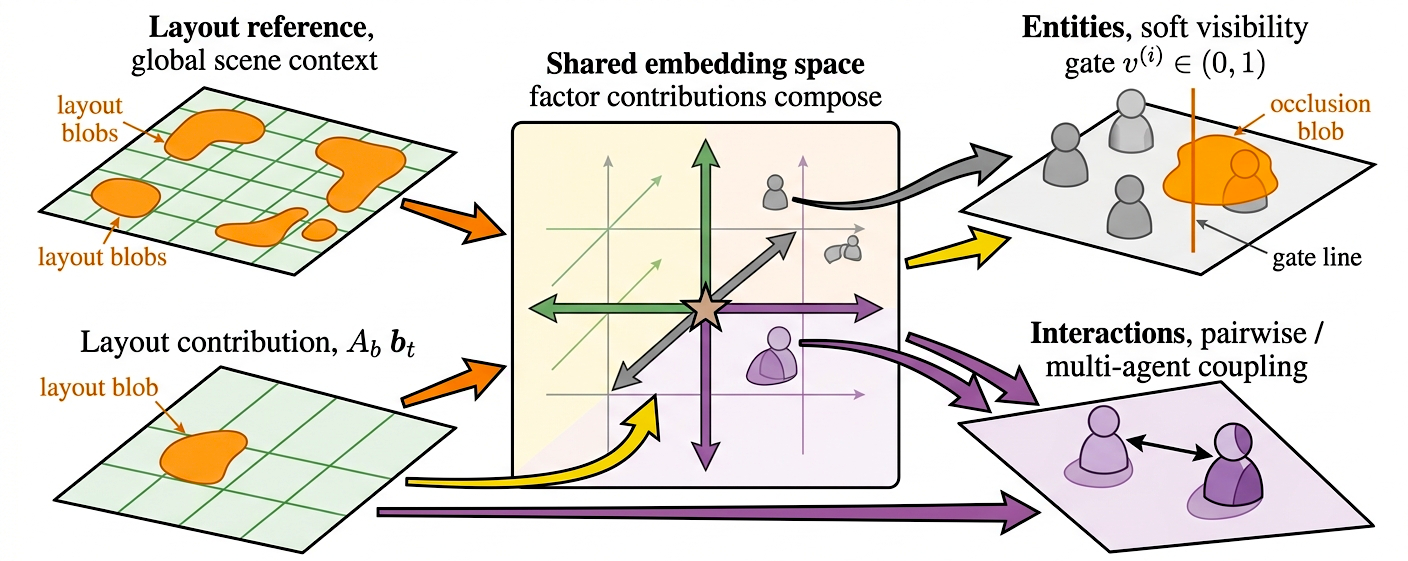
\includegraphics[width=\linewidth]{figures/factor_visual.png}
        \captionof{figure}{
\textbf{\emph{Factorized predictive channels.}}
Context is decomposed into \textbf{\emph{layout}}, visibility-gated
\textbf{\emph{agent}}, and sparse \textbf{\emph{interaction}} coordinates,
then composed in the future JEPA embedding. Separate subspaces preserve spatial
structure, partially observed agents, and multi-agent coupling while limiting
cross-factor leakage.
}
        \label{fig:factorjepa_visual}
    \end{minipage}
    \hfill
    \begin{minipage}[t]{0.48\textwidth}
        \centering
        
\includegraphics[width=0.85\linewidth]{figures/segmented_scene.png}
        \captionof{figure}{
        \textbf{\emph{DINO-based automatic factor-target construction.}}
        From each input clip, the pipeline derives complementary supervision
        for \textbf{\emph{layout}} $D_L$ by suppressing foreground agents,
        \textbf{\emph{agents}} $D_A$ by suppressing background context, and
        \textbf{\emph{interactions}} $D_I$ through temporally associated agent
        tubes. These targets semantically anchor FactorJEPA's predictive
        channels.
        }
        \label{fig:dino_factor_targets}
    \end{minipage}

    \vspace{-0.5em}
\end{figure*}


\section{\textbf{\emph{FactorJEPA}: Explicitly Factorized Predictive Channels}}
\label{sec:factorjepa}

\paragraph{\textbf{\emph{Motivation.}}}
Let $x$ be a video clip, $M_c$ and $M_t$ its context and target masks,
$f_\theta$ the online encoder, and $\bar f_{\bar\theta}$ the momentum target
encoder. The context representation and stop-gradient future target are

\begin{equation*}
\resizebox{0.98\columnwidth}{!}{$\displaystyle
h_t=f_\theta(M_c\odot x),
\qquad
Y_{t+\Delta}^{\star}
=
\operatorname{sg}\!\left(
\Pi_{M_t}[\bar f_{\bar\theta}(x)]
\right)
\in\mathbb{R}^{m\times d}
$}
\end{equation*}

where $\Pi_{M_t}$ denotes the executed target-selection operator, $m$ the
number of target representations, and $d$ their embedding dimension. A
conventional JEPA predictor learns

\begin{equation*}
g_\phi:(h_t,M_t)
\longmapsto
\widehat{Y}_{t+\Delta}
\in\mathbb{R}^{m\times d}
\end{equation*}

by matching $\widehat{Y}_{t+\Delta}$ to $Y_{t+\Delta}^{\star}$. The objective
specifies \emph{what} to predict, but leaves \emph{how predictive information
is internally organized} unconstrained.

This ambiguity is consequential in \textbf{DENSEWORLD}, where layout, agent
density, visibility, and interaction pressure are strongly correlated. A
high-capacity predictor can exploit \textbf{\emph{shortcut mixtures}}---crowd
texture as a proxy for interaction, visible appearance for object persistence,
or road geometry for motion---without recovering the structure governing scene
evolution.

\textbf{\emph{FactorJEPA}} resolves this ambiguity by replacing the monolithic
predictor with explicit \textbf{\emph{layout}}, \textbf{\emph{agent}}, and
\textbf{\emph{interaction}} channels. A \textbf{\emph{soft visibility gate}}
attenuates uncertain observations, while block-structured regularization limits
\textbf{\emph{cross-factor leakage}}. Together, these components factorize the
future JEPA embedding into semantically anchored coordinates and
factor-specific predictive subspaces.














\subsection{\textbf{\emph{DINOv2-Based Factor-Target Construction}}}
\label{sec:factor_target_construction}

For each privacy-filtered clip $x_n$, DINOv2 extracts visual features that our
preprocessing pipeline converts into region-level predictions
\cite{oquab2024dinov2}:

\begin{equation*}
\resizebox{0.98\columnwidth}{!}{$\displaystyle
\mathcal P_n
=
\mathcal D_{\mathrm{pre}}
\left(
\mathcal F_{\mathrm{DINOv2}}(x_n)
\right)
=
\left\{
(m_{n,t}^{(i)},b_{n,t}^{(i)},u_{n,t}^{(i)},p_{n,t}^{(i)})
\right\}_{t,i}
$}
\end{equation*}

where $m_{n,t}^{(i)}$, $b_{n,t}^{(i)}$, $u_{n,t}^{(i)}$, and
$p_{n,t}^{(i)}\in[0,1]$ denote the mask, bounding box, visual descriptor,
and confidence of region $i$ at time $t$. A temporal association operator links
consistent regions into tracklets:

\begin{equation*}
\mathcal A(\mathcal P_n)
=
\left\{
\tau_n^{(i)}
=
(m_{n,t}^{(i)},b_{n,t}^{(i)},u_{n,t}^{(i)})
_{t=t_s^{(i)}}^{t_e^{(i)}}
\right\}_{i}
\end{equation*}

A deterministic structural map converts region geometry, temporal continuity,
visibility, and relative motion into factor targets and reliability weights:

\begin{equation*}
\resizebox{0.98\columnwidth}{!}{$\displaystyle
\Psi_{\mathrm{struct}}
\left(
\mathcal P_n,\mathcal A(\mathcal P_n)
\right)
\longmapsto
\left\{
(T_{n,k},q_{n,k})
\right\}_{k\in\{L,A,V,I\}}
$}
\end{equation*}

Here, $T_{n,L}$, $T_{n,A}$, $T_{n,V}$, and $T_{n,I}$ encode layout, agents,
visibility, and tracklet-derived interactions. Each reliability weight
$q_{n,k}$ combines region confidence and temporal consistency. Using the factor
coordinates introduced next, factor-specific heads
$\widehat T_{n,k}=P_k(Z_{n,k})$ are trained with

\begin{equation*}
\mathcal L_{\mathrm{factor}}
=
\sum_{k\in\{L,A,I\}}
\frac{
\sum_{n=1}^{N}
q_{n,k}\,
\ell_k(\widehat T_{n,k},T_{n,k})
}{
\epsilon+\sum_{n=1}^{N}q_{n,k}
}
\end{equation*}

Visibility is optimized separately through $\mathcal L_v$. Thresholds are fixed
before evaluation, and low-confidence targets are excluded only from
factor-level diagnostics. DINOv2-derived targets are used only for training; no DINOv2 prediction,
tracklet, confidence, or postprocessed factor target is used as an evaluation
label. The exact DINOv2 checkpoint, preprocessing,
association and interaction rules, thresholds, per-factor coverage, and
reliability audit are reported in Appendix~\ref{app:annotation_protocol}.








\begin{figure*}[t]
    \centering

    \begin{minipage}[t]{0.48\textwidth}
        \centering
        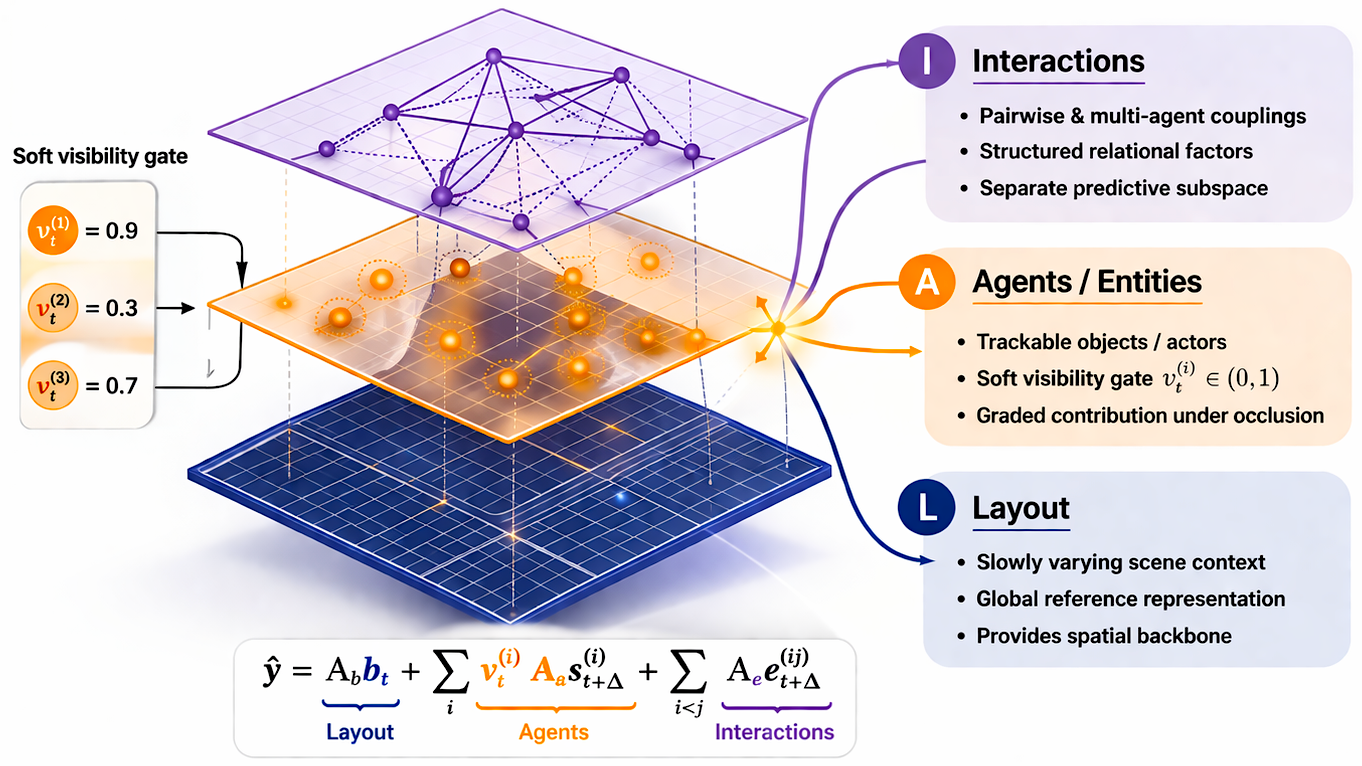
\includegraphics[width=\linewidth]{figures/factors.png}
        \vspace{-1.5em}
        \captionof{figure}{
        \textbf{\emph{Factorized prediction.}}
        \textbf{\emph{FactorJEPA}} composes the target embedding from
        \textbf{\emph{layout}}, \textbf{\emph{agents}}, and
        \textbf{\emph{interactions}}, with a soft visibility gate applied only to
        entity terms.
        }
        \label{fig:factorjepa_factors}
    \end{minipage}
    \hfill
    \begin{minipage}[t]{0.48\textwidth}
        \centering
        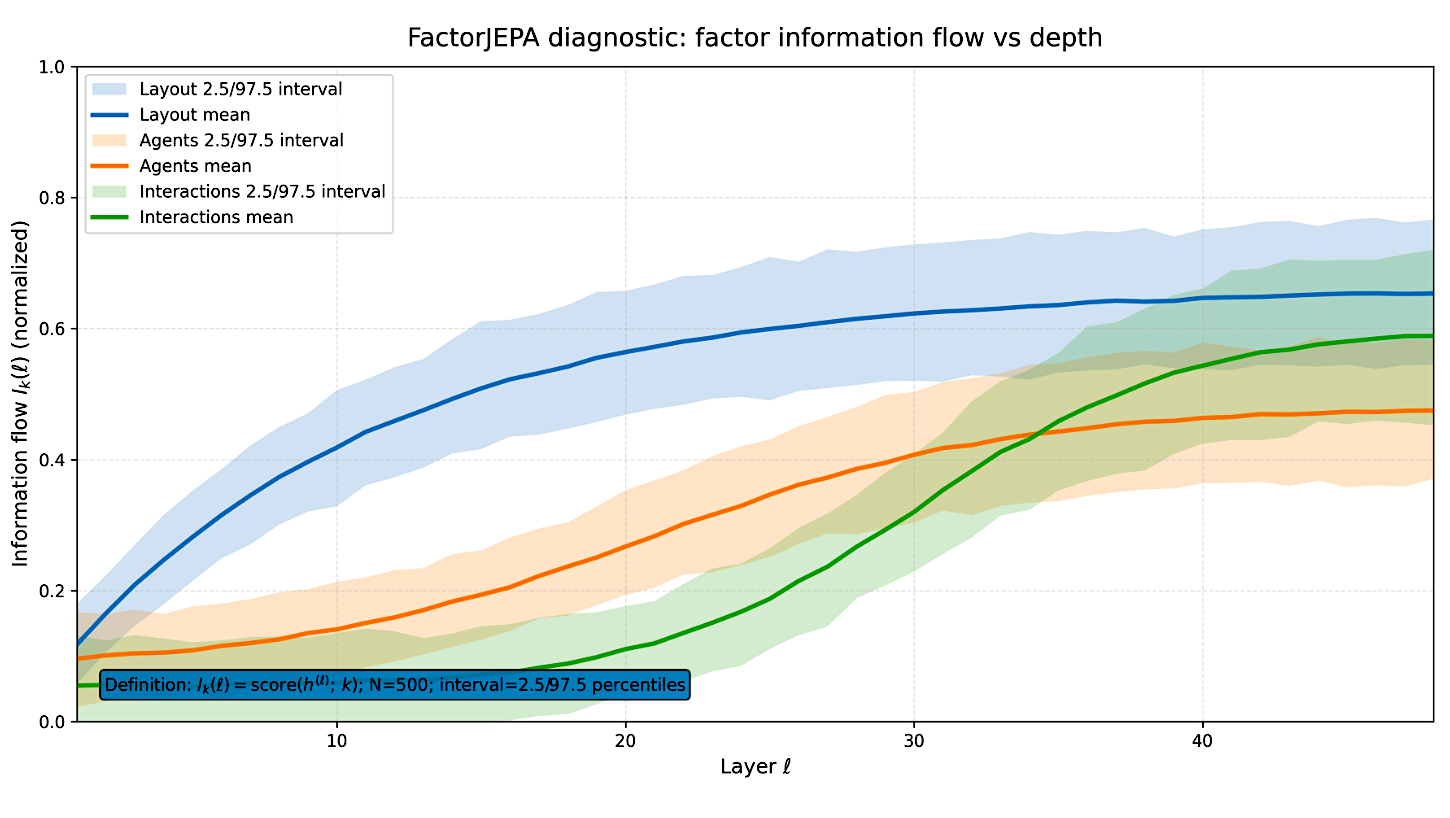
\includegraphics[width=\linewidth]{figures/factor_channels_depth.png}
        \vspace{-1.5em}
        \captionof{figure}{
        \textbf{\emph{Depth-wise factor realization.}}
        Lightweight probes show a staged profile: \textbf{\emph{layout}}
        emerges early, \textbf{\emph{agents}} grow gradually, and
        \textbf{\emph{interactions}} peak in deeper layers.
        }
        \label{fig:factorjepa_channels}
    \end{minipage}

    \vspace{-0.8em}
\end{figure*}










\subsection{\textbf{\emph{Structured Factor Coordinates}}}

For clip $x_n$, let $p\in\{1,\ldots,m\}$ index a target token and
$\pi_p$ denote its positional encoding. FactorJEPA first forms a
target-conditioned query

\begin{equation*}
q_{n,p}
=
Q\!\left(h_n,\pi_p,M_t\right),
\qquad
h_n=f_\theta(M_c\odot x_n),
\end{equation*}

and predicts three coordinate blocks for that target position:

\begin{equation*}
c_{n,p}
=
\operatorname{col}
\left(
c_{n,L,p},c_{n,A,p},c_{n,I,p}
\right)
\in
\mathbb{R}^{r_L+r_A+r_I}.
\end{equation*}

For readability, the target index $p$ is suppressed in the branch equations
below: $c_{n,k}$ denotes $c_{n,k,p}$ and each occurrence of $h_n$ denotes the
target-conditioned query $q_{n,p}$. The same factor branches are shared across
all target positions.

\paragraph{\textbf{\emph{Layout coordinates.}}}
The layout branch extracts slowly varying spatial support directly from the
global context:

\begin{equation*}
c_{n,L}
=
g_L(h_n)
\in\mathbb{R}^{r_L}.
\end{equation*}

It is supervised by the DINOv2-derived layout target $T_{n,L}$ through

\begin{equation*}
\widehat T_{n,L}
=
P_L(c_{n,L}).
\end{equation*}

\paragraph{\textbf{\emph{Visibility-gated agent coordinates.}}}
Let $o_n^{(i)}$ denote the representation of agent $i$, and let

\begin{equation*}
S_n
=
\left\{
s_n^{(i)}
\right\}_{i=1}^{N_n^A},
\qquad
s_n^{(i)}
=
g_A(h_n,o_n^{(i)})
\in\mathbb{R}^{r_A}
\end{equation*}

denote the object-centric agent states. FactorJEPA predicts a soft visibility
gate

\begin{equation*}
v_n^{(i)}
=
\sigma
\left(
g_V(h_n,o_n^{(i)})
\right)
\in(0,1).
\end{equation*}

The aggregated agent coordinate is

\begin{equation*}
c_{n,A}
=
\frac{
\sum_{i=1}^{N_n^A}
v_n^{(i)}s_n^{(i)}
}{
\epsilon+\sum_{i=1}^{N_n^A}v_n^{(i)}
}.
\end{equation*}

The normalization limits sensitivity to the number of detected agents, while
the gate attenuates uncertain or occluded observations without hard removal.

Given DINOv2-derived visibility targets $T_{n,V}^{(i)}$ and reliabilities
$q_{n,V}^{(i)}$, the gate loss is

\begin{equation*}
\resizebox{0.98\columnwidth}{!}{$\displaystyle
\mathcal L_v
=
-\frac{
\sum_{n,i}
q_{n,V}^{(i)}
\left[
T_{n,V}^{(i)}\log v_n^{(i)}
+
\left(1-T_{n,V}^{(i)}\right)
\log\left(1-v_n^{(i)}\right)
\right]
}{
\epsilon+\sum_{n,i}q_{n,V}^{(i)}
}
$}
\end{equation*}

\paragraph{\textbf{\emph{Sparse interaction coordinates.}}}
For each candidate pair $(i,j)\in\mathcal E_n$, the interaction branch predicts

\begin{equation*}
e_n^{(ij)}
=
g_I\!\left(h_n,o_n^{(i)},o_n^{(j)}\right),
\qquad
\bar e_n^{(ij)}
=
\frac{e_n^{(ij)}}
{\epsilon+\|e_n^{(ij)}\|_2}
\in\mathbb{R}^{r_I},
\end{equation*}

together with a soft interaction strength

\begin{equation*}
w_n^{(ij)}
=
\sigma\!\left(
g_W\!\left(h_n,o_n^{(i)},o_n^{(j)}\right)
\right)
\in(0,1).
\end{equation*}

Let $M_n=\max\{1,|\mathcal E_n|\}$. The interaction coordinate is

\begin{equation*}
c_{n,I}
=
\frac{1}{M_n}
\sum_{(i,j)\in\mathcal E_n}
w_n^{(ij)}\bar e_n^{(ij)},
\qquad
c_{n,I}=0
\ \text{if}\ 
\mathcal E_n=\varnothing.
\end{equation*}

A sparsity penalty encourages localized interactions:

\begin{equation*}
\mathcal L_{\mathrm{sparse}}
=
\frac{1}{N}
\sum_{n=1}^{N}
\frac{1}{M_n}
\sum_{(i,j)\in\mathcal E_n}
w_n^{(ij)}.
\end{equation*}

The fixed denominator removes weight-scale invariance: shrinking all
$w_n^{(ij)}$ now shrinks $c_{n,I}$ and cannot reduce the sparsity loss while
preserving the prediction. Normalizing $e_n^{(ij)}$ prevents compensation
through interaction-state magnitude.















\subsection{\textbf{\emph{Block-Structured Matrix Factorization}}}

For a minibatch of $N$ clips, stack the factor coordinates as

\begin{equation*}
\resizebox{0.98\columnwidth}{!}{$\displaystyle
C_k
=
\begin{bmatrix}
(c_{1,k,1})^\top\\
\vdots\\
(c_{1,k,m})^\top\\
\vdots\\
(c_{N,k,m})^\top
\end{bmatrix}
\in\mathbb{R}^{Nm\times r_k},
\qquad
k\in\{L,A,I\}.
$}
\end{equation*}

and concatenate the three blocks:

\begin{equation*}
C
=
\begin{bmatrix}
C_L&C_A&C_I
\end{bmatrix}
\in\mathbb{R}^{Nm\times r}.
\end{equation*}

Let $A_L$, $A_A$, and $A_I$ be learned synthesis dictionaries,

\begin{equation*}
\resizebox{0.98\columnwidth}{!}{$\displaystyle
A_k\in\mathbb{R}^{d\times r_k},
\qquad
A
=
\begin{bmatrix}
A_L&A_A&A_I
\end{bmatrix}
\in\mathbb{R}^{d\times r},
\qquad
k\in\{L,A,I\}
$}
\end{equation*}

that map the factor coordinates into the $d$-dimensional JEPA target space.
FactorJEPA predicts the complete minibatch target matrix through

\begin{equation*}
\resizebox{0.98\columnwidth}{!}{$\displaystyle
\boxed{
\widehat Y
=
\underbrace{
\begin{bmatrix}
C_L&C_A&C_I
\end{bmatrix}
}_{\text{world-factor coordinates}}
\underbrace{
\begin{bmatrix}
A_L&A_A&A_I
\end{bmatrix}^{\!\top}
}_{\text{predictive dictionaries}}
=
CA^\top
}
$}
\end{equation*}

This structured product is the defining FactorJEPA factorization. The row
factor $C$ specifies how each clip activates the layout, agent, and interaction
coordinates, while the columns of $A$ assign those coordinates predictive
directions in embedding space. Because each block is produced by a distinct
pathway, receives factor-specific supervision, and uses its own dictionary,
the factorization is architectural rather than a post-hoc partition.

Its block expansion is

\begin{equation*}
\widehat Y
=
\underbrace{C_LA_L^\top}_{Y_L}
+
\underbrace{C_AA_A^\top}_{Y_A}
+
\underbrace{C_IA_I^\top}_{Y_I}
\end{equation*}

where $Y_L$, $Y_A$, and $Y_I$ are the induced layout, agent, and interaction
contributions. For consistency with the clip-level factor coordinates, let

\begin{equation*}
Y^\star
=
\operatorname{col}
\left(
Y_{1,t+\Delta}^\star,
\ldots,
Y_{N,t+\Delta}^\star
\right)
\in\mathbb{R}^{Nm\times d}.
\end{equation*}

The token-level JEPA objective is therefore

\begin{equation*}
\mathcal L_{\mathrm{JEPA}}
=
\frac{1}{Nm}
\left\|
\widehat Y-Y^\star
\right\|_F^2.
\end{equation*}

For clip $x_n$, the corresponding $m$ rows of $\widehat Y$ are unstacked as

\begin{equation*}
\widehat Y_{n,t+\Delta}
=
\operatorname{Unstack}_n(\widehat Y)
\in\mathbb{R}^{m\times d}.
\end{equation*}

Thus, FactorJEPA preserves the complete target-token geometry: the factorization
operates over all $m$ future tokens, while pooling is used only for diagnostics
that explicitly require a clip-level representation.















\begin{figure*}[ht!]
    \centering
    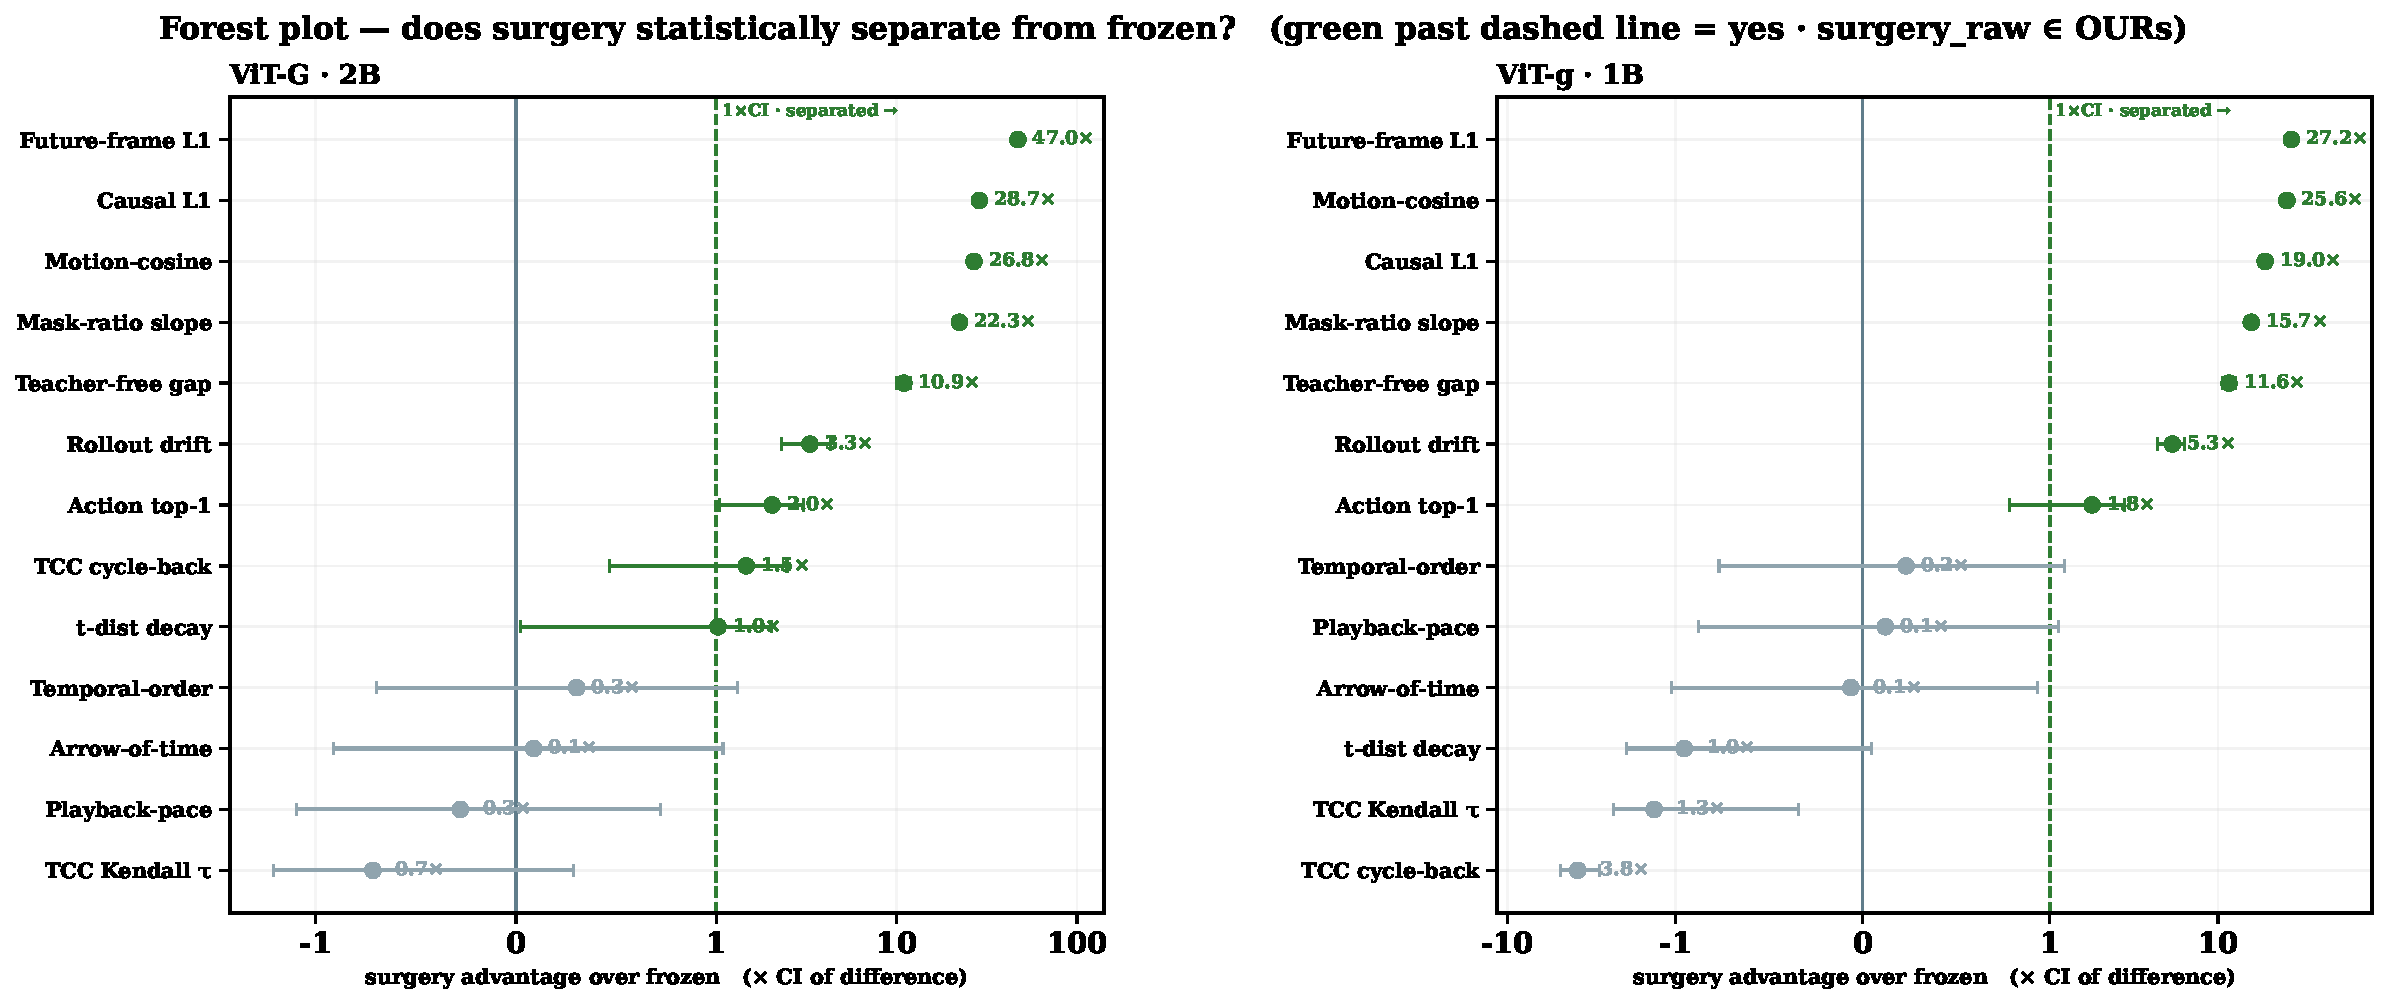
\includegraphics[width=0.95\textwidth]
    {figures/forest_plot_frozen_ci.pdf}
    \caption{
    \textbf{\emph{FactorJEPA separates decisively from the frozen backbone.}}
    Points report the signed advantage over frozen in units of the 95\%
    confidence interval of the paired difference; the dashed line marks
    statistical separation at $1\times$. FactorJEPA separates on all four
    headline diagnostics at both scales, reaching $47.0\times$ for
    Future-frame L1 at 2B and $27.2\times$ at 1B. These values measure
    confidence-interval separation, not multiplicative performance gains.
    }
    \label{fig:frozen_forest}
    \vspace{-0.6em}
\end{figure*}


\subsection{\textbf{\emph{Semantic Anchoring and Factor Ambiguity}}}

The factorization $\widehat Y=CA^\top$ is not unique. For any invertible
$R\in\mathbb{R}^{r\times r}$,

\begin{equation*}
CA^\top
=
(CR)
\left(
AR^{-\top}
\right)^\top
\end{equation*}

Thus, the JEPA objective alone permits rotations, cross-block mixing, and
permutations without changing the predicted target. It cannot assign operational
meaning to $C_L$, $C_A$, and $C_I$.

FactorJEPA anchors each block through a factor-specific head. For
$P_k\in\mathbb{R}^{p_k\times r_k}$,

\begin{equation*}
\widehat T_k
=
C_kP_k^\top
\in\mathbb{R}^{N\times p_k},
\qquad
k\in\{L,A,I\}
\end{equation*}

The corresponding confidence-normalized objective is

\begin{equation*}
\mathcal L_{\mathrm{factor}}
=
\sum_{k\in\{L,A,I\}}
\frac{
\sum_{n=1}^{N}
q_{n,k}\,
\ell_k(\widehat T_{n,k},T_{n,k})
}{
\epsilon+\sum_{n=1}^{N}q_{n,k}
}
\end{equation*}

This supervision assigns the blocks to layout, agents, and interactions,
restricting cross-factor mixing. Invertible transformations within each block
remain admissible; FactorJEPA therefore claims semantic block separation, not
coordinate-level identifiability.
















\subsection{\textbf{\emph{Block-Diagonal Channel Separation}}}

Explicit blocks do not guarantee separated information: different channels may
still encode correlated shortcuts. Let

\begin{equation*}
\resizebox{0.98\columnwidth}{!}{$\displaystyle
H_N
=
I_N-\frac{1}{N}\mathbf 1_N\mathbf 1_N^\top,
\qquad
\mathcal Y
=
\begin{bmatrix}
Y_L&Y_A&Y_I
\end{bmatrix}
\in\mathbb{R}^{N\times 3d}
$}
\end{equation*}

denote the minibatch-centering matrix and concatenated channel outputs. Their
empirical block covariance is

\begin{equation*}
\resizebox{0.98\columnwidth}{!}{$\displaystyle
\Gamma
=
\frac{1}{N-1}
\mathcal Y^\top H_N\mathcal Y,
\qquad
\Gamma_{kk'}
=
\frac{1}{N-1}
Y_k^\top H_NY_{k'},
\quad
k,k'\in\{L,A,I\}
$}
\end{equation*}

Diagonal blocks encode within-channel covariance, while off-diagonal blocks
measure second-order leakage across predictive channels. We penalize the
off-block component:

\begin{equation*}
\boxed{
\mathcal L_{\mathrm{cov}}
=
\left\|
\Gamma-
\operatorname{blkdiag}
\left(
\Gamma_{LL},\Gamma_{AA},\Gamma_{II}
\right)
\right\|_F^2.
}
\end{equation*}

Equivalently,

\begin{equation*}
\mathcal L_{\mathrm{cov}}
=
2\!\!
\sum_{\substack{k<k'\\k,k'\in\{L,A,I\}}}
\left\|
\Gamma_{kk'}
\right\|_F^2.
\end{equation*}

The objective leaves within-channel covariance unpenalized while suppressing
pairwise cross-channel covariance. It encourages operational factor separation,
but does not imply statistical or causal independence.


\paragraph{\textbf{\emph{Nonlinear leakage suppression.}}}
Cross-covariance controls only linear dependence. We additionally penalize
nonlinear dependence using normalized kernel alignment. For channel
$k\in\{L,A,I\}$, define an RBF Gram matrix over the minibatch:

\begin{equation*}
(K_k)_{ab}
=
\exp\!\left(
-\frac{\|Y_k^{(a)}-Y_k^{(b)}\|_2^2}{2\sigma_k^2}
\right),
\qquad
\bar K_k=H_NK_kH_N,
\end{equation*}

where $\sigma_k$ is the stop-gradient median pairwise distance within channel
$k$. The nonlinear dependence penalty is

\begin{equation*}
\mathcal L_{\mathrm{nlin}}
=
\sum_{\substack{k<k'\\k,k'\in\{L,A,I\}}}
\frac{
\operatorname{tr}\!\left(\bar K_k\bar K_{k'}\right)
}{
\|\bar K_k\|_F\|\bar K_{k'}\|_F+\epsilon
}.
\end{equation*}

The complete separation objective is

\begin{equation*}
\boxed{
\mathcal L_{\mathrm{sep}}
=
\mathcal L_{\mathrm{cov}}
+
\beta_{\mathrm{nlin}}\mathcal L_{\mathrm{nlin}}.
}
\end{equation*}

Thus, $\mathcal L_{\mathrm{cov}}$ suppresses linear cross-channel leakage,
while $\mathcal L_{\mathrm{nlin}}$ discourages dependence detectable in a
characteristic-kernel feature space. The JEPA and factor-supervision losses
preserve predictive variation within each channel; separation is applied only
across channels.


















\subsection{\textbf{\emph{Cross-Factor Leakage Diagnostic}}}

Separation losses do not by themselves establish factor specificity. We
therefore freeze FactorJEPA and train fixed-capacity nonlinear probes
$r_{k\rightarrow k'}$ to predict target $T_{k'}$ from channel $Y_k$:

\begin{equation*}
\resizebox{0.98\columnwidth}{!}{$\displaystyle
r_{k\rightarrow k'}
=
\arg\min_r
\sum_{n\in\mathcal D_{\mathrm{train}}}
\ell_{k'}\!\left(
r(Y_{n,k}),T_{n,k'}
\right),
\qquad
k,k'\in\{L,A,I\}.
$}
\end{equation*}

Let $S_{k\rightarrow k'}$ denote the corresponding held-out score and
$S_{0\rightarrow k'}$ the score of a constant predictor. We report normalized
cross-factor leakage as

\begin{equation*}
\operatorname{Leak}(k\!\rightarrow\!k')
=
\frac{
S_{k\rightarrow k'}-S_{0\rightarrow k'}
}{
S_{k'\rightarrow k'}-S_{0\rightarrow k'}+\epsilon
},
\qquad
k\neq k'.
\end{equation*}

A well-separated representation should retain strong diagonal predictability
$S_{k\rightarrow k}$ while exhibiting low off-diagonal leakage. Probes are
trained only on the training split and evaluated on held-out clips.








\begin{figure*}[ht!]
    \centering
    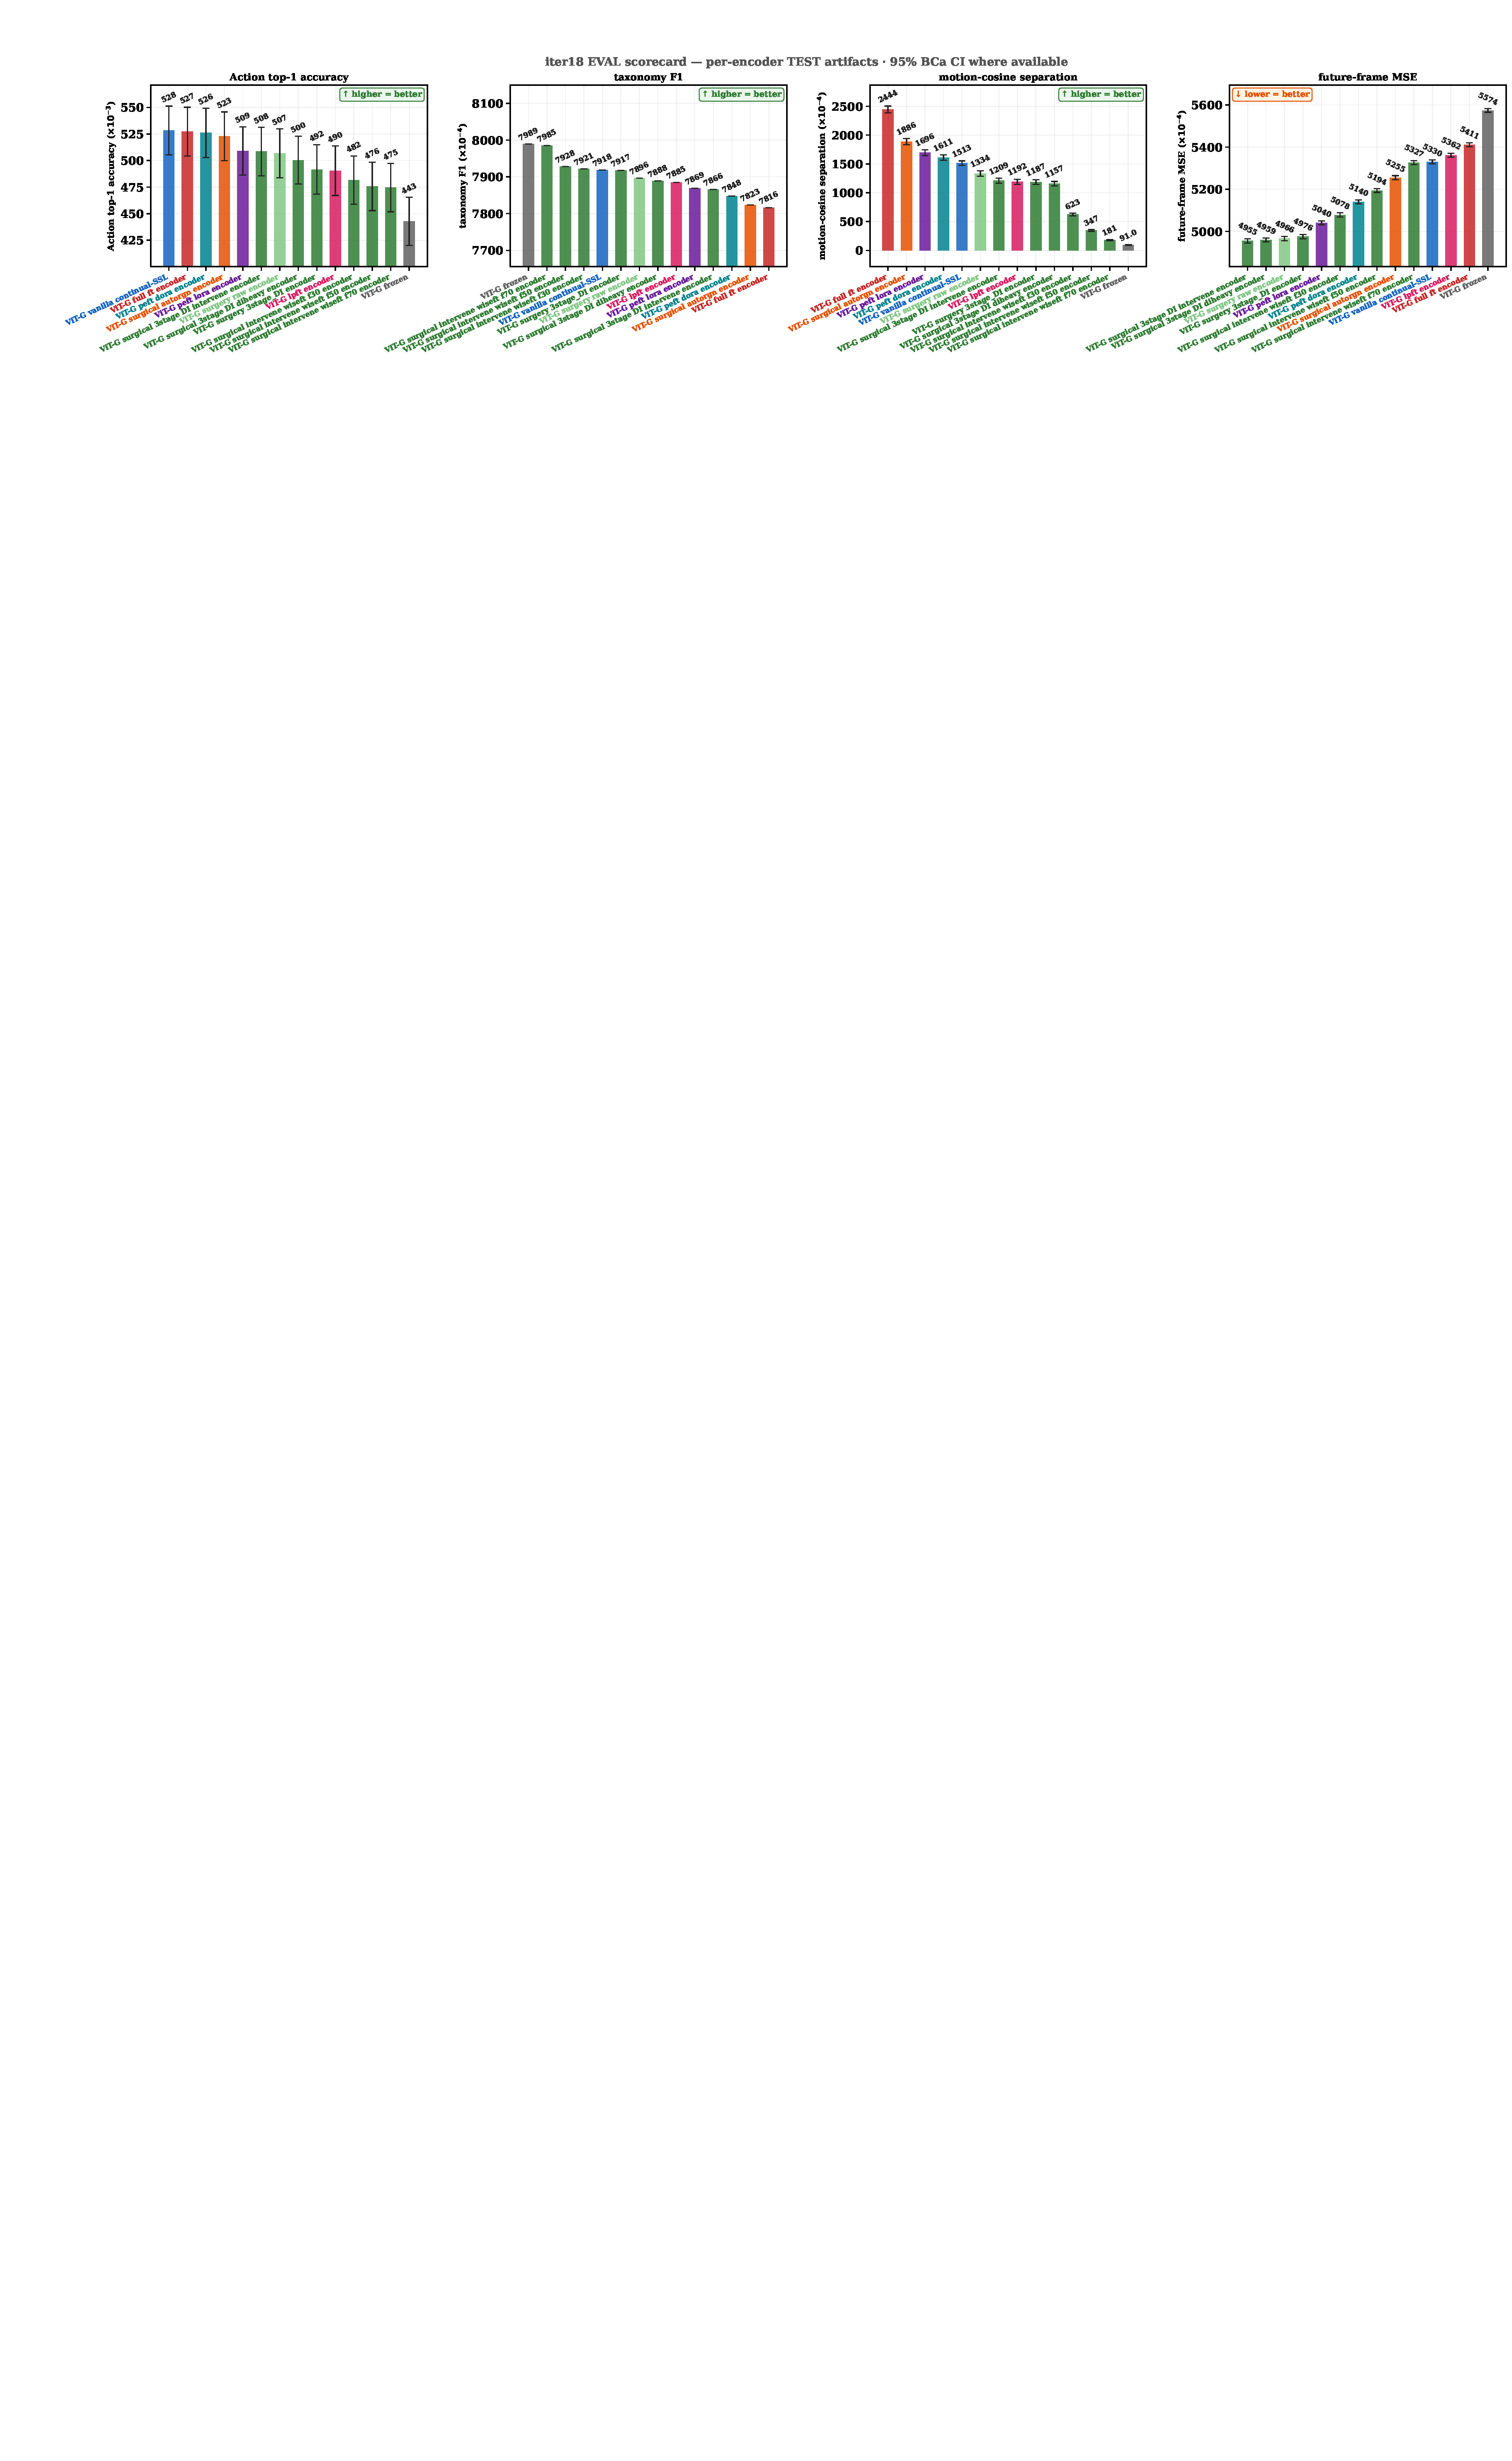
\includegraphics[width=\textwidth]
    {figures/eval_scorecard_combined_one_row.pdf}
    \caption{
    \textbf{\emph{Complete evaluation scorecard at 2B and 1B scales.}}
    We compare frozen, conventionally adapted, parameter-efficient, and
    factorized V-JEPA~2.1 variants across 15 semantic, predictive, motion, and
    temporal-coherence diagnostics. Bars report test performance with 95\% BCa
    confidence intervals where available. The four headline diagnostics are
    Future-frame L1, Causal L1, Motion cosine, and Mask-ratio slope.
    }
    \label{fig:eval_scorecard}
    \vspace{-0.6em}
\end{figure*}


\begin{figure*}[ht!]
    \centering
    
\includegraphics[width=\textwidth]
    {figures/scale_replication.pdf}
    \caption{
    \textbf{\emph{Method rankings replicate from 2B to 1B.}}
    Each panel compares complete per-method scores at the two scales; titles
    report Spearman rank correlation. The four headline diagnostics replicate
    most strongly: Causal L1 ($\rho=0.978$), Motion cosine
    ($\rho=0.952$), Future-frame L1 ($\rho=0.938$), and Mask-ratio slope
    ($\rho=0.895$). Three secondary diagnostics do not transfer and are shown
    in red.
    }
    \label{fig:scale_replication}
    \vspace{-0.6em}
\end{figure*}



\subsection{\textbf{\emph{Predictor Surgery}}}

FactorJEPA is initialized from a pretrained V-JEPA model. The online encoder,
momentum target encoder, target construction, and masking policy are retained.
Only the monolithic predictor is replaced:

\begin{equation*}
\Theta_{\mathrm{pred}}
\longrightarrow
\Theta_{\mathrm{fact}}
=
\left\{
\Theta_L,\Theta_A,\Theta_I,\Theta_V,\Theta_W,A
\right\}.
\end{equation*}

Training is restricted to the factorized predictor and the top $K$ encoder
blocks:

\begin{equation*}
\Theta_{\mathrm{train}}
=
\Theta_{\mathrm{fact}}
\cup
\Theta_{\mathrm{top}\text{-}K}.
\end{equation*}

The lower encoder blocks and momentum target network follow the frozen or
momentum-updated protocol of the underlying V-JEPA implementation.

The final objective is
\begin{equation*}
\boxed{
\begin{aligned}
\mathcal L
&=
\mathcal L_{\mathrm{JEPA}}
+
\lambda_{\mathrm{sep}}\mathcal L_{\mathrm{sep}}
+
\lambda_{\mathrm{sparse}}\mathcal L_{\mathrm{sparse}}\\
&\quad+
\lambda_v\mathcal L_v
+
\lambda_{\mathrm{sup}}\mathcal L_{\mathrm{factor}}.
\end{aligned}
}
\end{equation*}

Each term has a distinct role:
\begin{equation*}
\begin{array}{rcl}
\mathcal L_{\mathrm{JEPA}}
&:&
\text{future-latent prediction},\\
\mathcal L_{\mathrm{sep}}
&:&
\text{cross-channel leakage suppression},\\
\mathcal L_{\mathrm{sparse}}
&:&
\text{interaction locality},\\
\mathcal L_v
&:&
\text{visibility calibration},\\
\mathcal L_{\mathrm{factor}}
&:&
\text{semantic anchoring}.
\end{array}
\end{equation*}






\subsection{\textbf{\emph{Depth-Wise Factor Realization}}}
\label{sec:depth_analysis}

Although the factorization acts at the predictor, we test how factor information
becomes linearly accessible across encoder depth. Let

\begin{equation*}
H^{(\ell)}
=
\begin{bmatrix}
h_1^{(\ell)}&\cdots&h_N^{(\ell)}
\end{bmatrix}^{\!\top}
\in\mathbb{R}^{N\times d_\ell}
\end{equation*}

denote the representations at layer $\ell$. For each factor
$k\in\{L,A,I\}$, we fit a regularized linear probe on the training split:

\begin{equation*}
\resizebox{0.98\columnwidth}{!}{$\displaystyle
W_k^{(\ell)}
=
\arg\min_W
\left\|
H_{\mathrm{train}}^{(\ell)}W-T_{k,\mathrm{train}}
\right\|_F^2
+
\lambda_{\mathrm{probe}}\|W\|_F^2
$}
\end{equation*}

The held-out depth-wise factor score is

\begin{equation*}
I_k(\ell)
=
\operatorname{score}_k
\left(
H_{\mathrm{test}}^{(\ell)}W_k^{(\ell)},
T_{k,\mathrm{test}}
\right).
\end{equation*}

Distinct onset and growth profiles indicate that layout, agent, and interaction
information becomes accessible at different depths. This is a representation
diagnostic, not a neuron-level or causal decomposition.















































\section{\textbf{Experiments \& Evaluation}}
\label{sec:experiments}

We evaluate whether FactorJEPA improves the predictive structure of V-JEPA
rather than only its downstream semantics. Our analysis centers on four
diagnostics: \textbf{Future-frame L1}, \textbf{Causal L1},
\textbf{Mask-ratio slope}, and \textbf{Motion cosine}. Together, they measure
future-latent accuracy, intervention sensitivity, robustness to missing visual
evidence, and linearly accessible motion information.


\subsection{\textbf{\emph{Evaluator Independence and Audit Split}}}
\label{sec:evaluator_independence}

To prevent agreement with the pseudo-label generator from being mistaken for
improved world modeling, we separate training-target construction from
evaluation. DINOv2-derived targets are constructed only on the training split:

\begin{equation*}
\mathcal T_{\mathrm{train}}
=
\Psi_{\mathrm{struct}}
\left(
\mathcal F_{\mathrm{DINOv2}}(x)
\right),
\qquad
x\in\mathcal D_{\mathrm{train}}.
\end{equation*}

Primary factor-specific evaluation is performed on a city-disjoint audit split
$\mathcal D_{\mathrm{audit}}$, whose agent masks, visibility states,
interaction pairs, and intervention regions are annotated independently:

\begin{equation*}
\mathcal D_{\mathrm{train}}
\cap
\mathcal D_{\mathrm{audit}}
=
\varnothing,
\qquad
\mathcal T_{\mathrm{audit}}
=
\Psi_{\mathrm{human}}(x).
\end{equation*}

The audit annotations are not used for training, model selection, threshold
selection, or hyperparameter tuning. Future-frame L1 and Mask-ratio slope use
only the frozen V-JEPA target encoder; Motion cosine uses an independently
frozen motion estimator; and RGB Agent F1 uses a frozen detector that supplies
neither FactorJEPA supervision nor DINOv2 preprocessing. Thus, no headline
metric reuses FactorJEPA's pseudo-label generator as its evaluator.

\subsection{\textbf{\emph{Protocol and Comparisons}}}

We evaluate V-JEPA~2.1 at two scales: ViT-G with approximately 2B parameters
and ViT-g with approximately 1B parameters. The comparison spans the frozen
backbone, conventional full and parameter-efficient fine-tuning, LoRA, DoRA,
Auto-RGN, \textbf{FactorJEPA-RAW}, and full \textbf{FactorJEPA}.
FactorJEPA-RAW applies the factorized predictor to raw clips without
factor-target supervision, separating architectural gains from those introduced
by the factor curriculum.

We additionally evaluate \textbf{FactorJEPA-RAW}, which applies the factorized predictor architecture to the same raw clips without factor-target supervision. The resulting attribution chain,
\begin{equation*}
\resizebox{0.98\columnwidth}{!}{$\displaystyle
\underbrace{\{\text{LoRA},\text{DoRA},\text{Auto-RGN}\}}_{\text{generic adaptation}}
\;\longrightarrow\;
\underbrace{\text{FactorJEPA-RAW}}_{\text{factorized architecture}}
\;\longrightarrow\;
\underbrace{\text{FactorJEPA}}_{\text{architecture + factor curriculum}}
$}
\end{equation*}
separates gains due to parameter adaptation, predictor structure, and structured supervision. Results in Section~\ref{sec:experiments} therefore test a precise claim: whether explicit \textbf{layout--agent--interaction structure} improves future prediction beyond the adaptation capacity of a monolithic JEPA predictor under a matched protocol.

All methods use the same clips, masking policy, evaluation split, and metric
implementations. We report per-encoder test results with 95\% BCa bootstrap
confidence intervals. In the exported evaluation figures,
\emph{surgery} denotes FactorJEPA and \emph{surgery-raw} denotes
FactorJEPA-RAW.


\begin{table}[ht!]
\centering
\caption{
\textbf{Training and evaluation provenance.}
No headline evaluator supplies FactorJEPA supervision.
}
\label{tab:evaluator_provenance}
\scriptsize
\setlength{\tabcolsep}{3pt}
\renewcommand{\arraystretch}{1.08}
\resizebox{\columnwidth}{!}{%
\begin{tabular}{lll}
\toprule
\textbf{Signal} & \textbf{Source} & \textbf{Factor-target source?} \\
\midrule
Factor supervision       & DINOv2 pipeline          & Yes \\
Audit factors/interventions & Human annotations     & No \\
Future latent            & Frozen target encoder    & No \\
Motion descriptor        & Frozen motion estimator  & No \\
RGB Agent F1             & Independent detector     & No \\
\bottomrule
\end{tabular}%
}
\vspace{-0.7em}
\end{table}




\subsection{\textbf{\emph{Four Diagnostics of Predictive Structure}}}

\paragraph{\textbf{\emph{Future-frame L1 ($\downarrow$).}}}
Normalized L1 distance between predicted and target future embeddings; lower
values indicate \textbf{\emph{more accurate future-latent prediction}}.

\paragraph{\textbf{\emph{Causal L1 ($\downarrow$).}}}
For each independently annotated intervention region $a$, we apply the same
controlled edit $\mathcal I_a$ to the evaluated clip and compare the resulting
change in predicted and target future latents:

\begin{equation*}
\resizebox{0.98\columnwidth}{!}{$\displaystyle
\widehat\Delta_a
=
\widehat Y\!\left(\mathcal I_a(x)\right)-\widehat Y(x),
\qquad
\Delta_a^\star
=
\operatorname{sg}\!\left[
\bar f_{\bar\theta}\!\left(\mathcal I_a(x)\right)
-
\bar f_{\bar\theta}(x)
\right].
$}
\end{equation*}

\begin{equation*}
\operatorname{CausalL1}
=
\frac{1}{|\mathcal A|}
\sum_{a\in\mathcal A}
\frac{
\|\widehat\Delta_a-\Delta_a^\star\|_1
}{
\epsilon+\|\Delta_a^\star\|_1
}.
\end{equation*}

Intervention regions and types are defined by the independent audit annotations,
not by DINOv2 predictions. This metric measures consistency with controlled
intervention-induced changes; it does not establish causal identification.

\paragraph{\textbf{\emph{Mask-ratio slope ($\downarrow$).}}}
The increase in prediction error as visual evidence is progressively masked; a
smaller slope indicates \textbf{\emph{greater robustness under partial
observability}}.

\paragraph{\textbf{\emph{Motion cosine ($\uparrow$).}}}
Cosine alignment between linearly decoded and target motion descriptors; higher
values indicate \textbf{\emph{more linearly accessible motion information}}.



\subsection{\textbf{\emph{Decisive Gains over the Frozen World Model}}}

Figure~\ref{fig:frozen_forest} reports FactorJEPA's advantage over the frozen
backbone in confidence-interval widths; values beyond $1\times$ indicate
statistical separation. FactorJEPA clears this threshold on
\textbf{\emph{all four headline diagnostics at both scales}}.

At 2B/1B, separation reaches
\textbf{\emph{$47.0\times$/$27.2\times$}} for Future-frame L1,
\textbf{\emph{$28.7\times$/$19.0\times$}} for Causal L1,
\textbf{\emph{$26.8\times$/$25.6\times$}} for Motion cosine, and
\textbf{\emph{$22.3\times$/$15.7\times$}} for Mask-ratio slope. These are
confidence-relative effect strengths, not multiplicative performance gains,
and remain decisive after scaling from 2B to 1B.

The full scorecard (Figure~\ref{fig:eval_scorecard}) shows a
\textbf{\emph{structured, not universal, gain}}: FactorJEPA leads on prediction,
intervention, masking, and motion-sensitive diagnostics, while frozen or
conventionally tuned models retain advantages on several frame-timing and
temporal-coherence measures.



\subsection{\textbf{\emph{Prediction--Motion Trade-off}}}

Against the strongest non-FactorJEPA adaptation, FactorJEPA improves
\textbf{\emph{Future-frame L1}} by 1.7\%/1.4\% at 2B/1B
($6.3\times$/$4.8\times$ CI widths),
\textbf{\emph{Causal L1}} by 0.9\%/1.1\%
($2.3\times$/$2.7\times$), and
\textbf{\emph{Mask-ratio slope}} by 1.1\%/2.9\%, although the 2B masking
result remains marginal.

The trade-off is \textbf{\emph{Motion cosine}}. FactorJEPA improves motion
accessibility over the frozen backbone, but trails the strongest full-fine-tuning
arm by 44.9\%/33.4\% at 2B/1B. Thus, factorization favors
\textbf{\emph{accurate, intervention-sensitive, and occlusion-robust
prediction}} over maximally linear motion readout---a trade-off that replicates
across scales.




\subsection{\textbf{\emph{Cross-Scale Replication}}}

We next ask whether the complete ranking of adaptation methods survives the
transition from the 2B backbone to the approximately half-cost 1B backbone.
For diagnostic $k$, we compute

\begin{equation*}
\rho_k
=
\operatorname{Spearman}
\left(
\mathbf s_k^{2\mathrm B},
\mathbf s_k^{1\mathrm B}
\right),
\end{equation*}

where $\mathbf s_k^{2\mathrm B}$ and $\mathbf s_k^{1\mathrm B}$ contain the
per-method scores at the two scales.



As Figure~\ref{fig:scale_replication} shows, Causal L1 yields
$\rho=0.978$, Motion cosine $\rho=0.952$, Future-frame L1
$\rho=0.938$, and Mask-ratio slope $\rho=0.895$. These are the four strongest
cross-scale correlations in the evaluation. Twelve of the fifteen diagnostics
retain broadly consistent rankings, while Temporal-order, Teacher-free gap,
and Rollout drift do not transfer reliably.

The replication result is important for two reasons. First, it shows that both
the predictive gains and the motion trade-off are stable properties of the
method ordering rather than artifacts of one backbone. Second, it establishes
the 1B model as a faithful lower-cost proxy for screening adaptation choices
before full-scale 2B training.

\paragraph{\textbf{\emph{Evaluation takeaway.}}}
Across both scales, FactorJEPA delivers
\textbf{\emph{(i) more accurate future-latent prediction}},
\textbf{\emph{(ii) stronger intervention-sensitive structure}}, and
\textbf{\emph{(iii) greater robustness under reduced visual evidence}}.
It also makes motion substantially more accessible than in the frozen world
model, while conceding motion linearity to the strongest generic fine-tuning
arm. These effects replicate with $\rho=0.895$--$0.978$, showing that explicit
factorization changes not only prediction error, but the structure and
accessibility of the information used to forecast the future.













































\section{\textbf{From Future Latents to Visible Futures}}
\label{sec:latent_to_rgb}

JEPA models predict in embedding space, making their forecasts difficult to
inspect directly. We therefore introduce a \textbf{\emph{Cosmos-initialized
latent-to-RGB decoder}} that renders FactorJEPA's predicted future embedding as
an RGB frame. The decoder does not perform forecasting or alter FactorJEPA; it
provides a visual interface to the future already predicted in latent space.

\subsection{\textbf{\emph{Latent Transport and RGB Decoding}}}

FactorJEPA produces a future embedding
$\widehat Y_{t+\Delta}\in\mathbb{R}^{m\times d_J}$, whereas the Cosmos decoder
expects a spatial conditioning tensor. We introduce a learned transport
operator

\begin{equation*}
\mathcal T_\omega:
\mathbb{R}^{m\times d_J}
\longrightarrow
\mathbb{R}^{h\times w\times d_C}
\end{equation*}

that aligns the JEPA token geometry, dimensionality, and feature statistics with
the Cosmos decoding space. The rendered future is

\begin{equation*}
\boxed{
\widehat x_{t+\Delta}
=
\mathcal G_{\psi_C}
\left(
\mathcal T_\omega(
\widehat Y_{t+\Delta})
\right)
}
\end{equation*}

where $\mathcal G_{\psi_C}$ is initialized from the corresponding Cosmos
component~\cite{nvidia2025cosmos}. At inference, the decoder receives only
FactorJEPA's predicted future latent; the ground-truth future frame is never
provided.





\begin{figure*}[ht!]
    \centering
    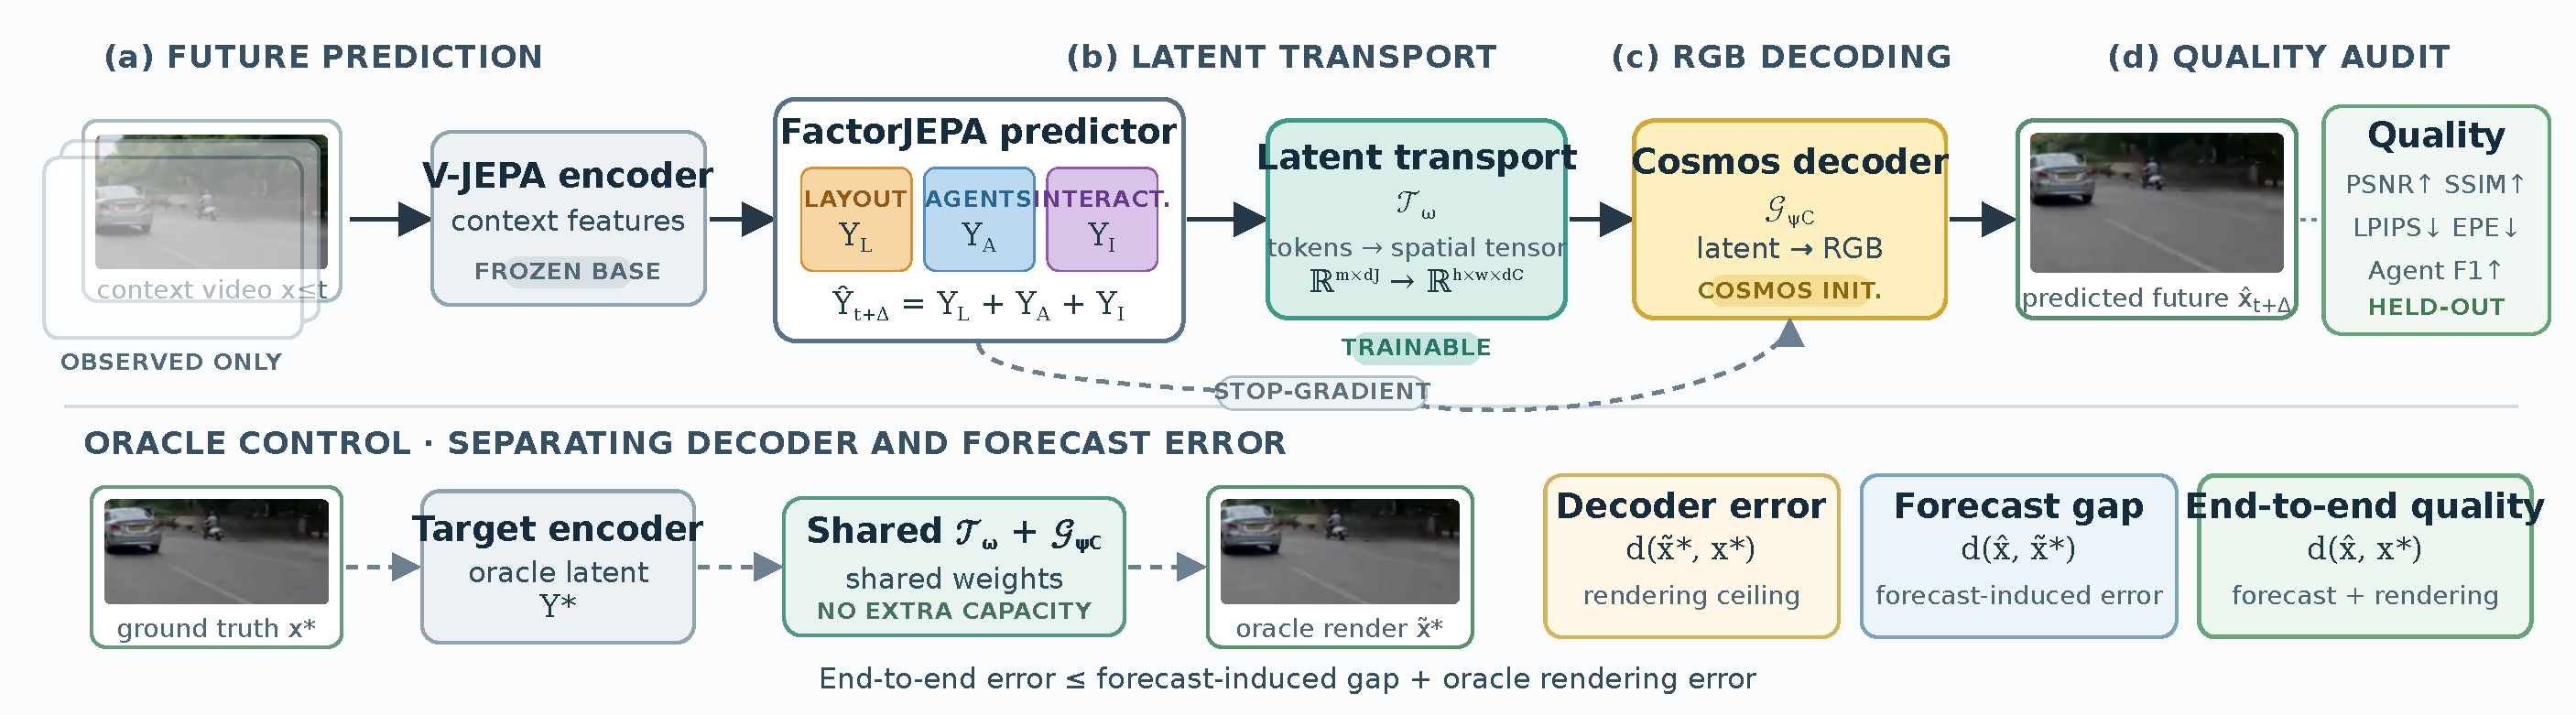
\includegraphics[width=\textwidth]
    {figures/latent_to_rgb_pipeline.pdf}
    \vspace{-0.6em}
    \caption{
    \textbf{\emph{From factorized future latents to visible futures.}}
    FactorJEPA predicts \textbf{\emph{layout}}, \textbf{\emph{agent}}, and
    \textbf{\emph{interaction}} channels, which a learned transport maps into
    the conditioning space of a \textbf{Cosmos-initialized decoder} to render
    the predicted future RGB frame. An oracle reconstruction from the target
    future latent separates \textbf{\emph{decoder error}} from the
    \textbf{\emph{forecast-induced gap}}, while their combination measures
    \textbf{\emph{end-to-end prediction quality}}. RGB reconstruction gradients
    are stopped before FactorJEPA.
    }
    \label{fig:latent_to_rgb_pipeline}
    \vspace{-1.0em}
\end{figure*}

\subsection{\textbf{\emph{Decoder Adaptation}}}

We first train the decoder to invert target-encoder latents. Let
$Y_{t+\Delta}^{\star}$ be the stop-gradient target latent paired with the
observed future frame $x_{t+\Delta}$. Its oracle reconstruction is

\begin{equation*}
\widetilde x_{t+\Delta}^{\star}
=
\mathcal G_{\psi_C}
\left(
\mathcal T_\omega(
Y_{t+\Delta}^{\star})
\right).
\end{equation*}

To reduce the distribution gap between target and predicted latents, the
decoder is additionally exposed to stop-gradient FactorJEPA predictions. The
training objective is

\begin{equation*}
\resizebox{0.98\columnwidth}{!}{$\displaystyle
\boxed{
\mathcal L_{\mathrm{decode}}
=
\mathbb E
\left[
\ell_{\mathrm{RGB}}
\left(
\widetilde x_{t+\Delta}^{\star},
x_{t+\Delta}
\right)
\right]
+
\eta\,
\mathbb E
\left[
\ell_{\mathrm{RGB}}
\left(
\widehat x_{t+\Delta},
x_{t+\Delta}
\right)
\right]
}
$}
\end{equation*}

FactorJEPA is frozen throughout decoder training, and
$\operatorname{sg}(\widehat Y_{t+\Delta})$ is used in the second term. Thus,
RGB reconstruction cannot modify the world model or its latent forecasts.
The executed reconstruction losses, Cosmos checkpoint, transport architecture,
latent normalization, and value of $\eta$ are reported in
Appendix~\ref{app:latent_rgb_details}.

\subsection{\textbf{\emph{Separating Forecast and Decoder Error}}}

A decoded prediction can fail because the future latent is inaccurate or
because the decoder cannot perfectly invert a correct latent. We separate these
sources using the oracle reconstruction:

\begin{equation*}
\begin{aligned}
\left\|
\widehat x_{t+\Delta}-x_{t+\Delta}
\right\|
&\le
\underbrace{
\left\|
\widehat x_{t+\Delta}
-
\widetilde x_{t+\Delta}^{\star}
\right\|
}_{\text{forecast-induced rendering gap}}
\\[-1mm]
&\quad+
\underbrace{
\left\|
\widetilde x_{t+\Delta}^{\star}
-
x_{t+\Delta}
\right\|
}_{\text{oracle decoder error}}.
\end{aligned}
\end{equation*}

The oracle term measures the decoder's reconstruction ceiling; the forecast
term measures the visible effect of replacing the target latent with
FactorJEPA's prediction. This decomposition prevents decoder limitations from
being attributed to the world model.

\subsection{\textbf{\emph{Evaluating RGB Prediction Quality}}}

We evaluate held-out reconstructions along five complementary axes:
\textbf{\emph{(i) pixel fidelity}} using PSNR,
\textbf{\emph{(ii) structural fidelity}} using SSIM,
\textbf{\emph{(iii) perceptual similarity}} using LPIPS,
\textbf{\emph{(iv) motion fidelity}} using optical-flow endpoint error, and
\textbf{\emph{(v) crowded-scene fidelity}} using agent F1 from a frozen,
independent evaluator. No evaluator used for RGB assessment supplies
FactorJEPA's factor targets.

For motion fidelity, let $x_t$ be the final context frame and define

\begin{equation*}
F^\star
=
\operatorname{Flow}(x_t,x_{t+\Delta}),
\qquad
\widehat F
=
\operatorname{Flow}(x_t,\widehat x_{t+\Delta}).
\end{equation*}

We report

\begin{equation*}
\operatorname{EPE}_{\mathrm{flow}}
=
\frac{1}{HW}
\sum_{p}
\left\|
\widehat F(p)-F^\star(p)
\right\|_2,
\end{equation*}

using the same frozen flow estimator for every method. This tests whether the
rendered future moves correctly, rather than only whether it appears realistic.

The evaluation compares four latent sources under the
\textbf{\emph{same decoder}}: target latents provide the oracle ceiling;
standard V-JEPA predictions test monolithic forecasting;
FactorJEPA-RAW isolates architectural factorization; and full FactorJEPA
measures architecture plus factor supervision.

\begin{table}[ht!]
\centering
\caption{
\textbf{Latent-to-RGB prediction on held-out clips.}
Oracle decoding isolates decoder capacity; predicted latents evaluate the
complete world-model--decoder pipeline. All methods share the same
Cosmos-initialized decoder.
}
\label{tab:latent_rgb}
\vspace{-0.4em}
\scriptsize
\setlength{\tabcolsep}{3pt}
\renewcommand{\arraystretch}{1.10}
\resizebox{\columnwidth}{!}{%
\begin{tabular}{lccccc}
\toprule
\textbf{Latent source}
& \shortstack{\textbf{PSNR}\\$\uparrow$}
& \shortstack{\textbf{SSIM}\\$\uparrow$}
& \shortstack{\textbf{LPIPS}\\$\downarrow$}
& \shortstack{\textbf{Flow EPE}\\$\downarrow$}
& \shortstack{\textbf{Agent F1}\\$\uparrow$} \\
\midrule
Target latent (oracle)    & -- & -- & -- & -- & -- \\
V-JEPA                    & -- & -- & -- & -- & -- \\
FactorJEPA-RAW            & -- & -- & -- & -- & -- \\
\textbf{FactorJEPA}       & -- & -- & -- & -- & -- \\
\bottomrule
\end{tabular}%
}
\vspace{-0.7em}
\end{table}

\subsection{\textbf{\emph{Factor-Level Visual Inspection}}}

The factorized prediction also enables controlled pixel-space inspection.
Writing

\begin{equation*}
\widehat Y
=
Y_L+Y_A+Y_I,
\end{equation*}

we decode a factor-removed future

\begin{equation*}
\widehat x^{(-k)}
=
\mathcal G_{\psi_C}
\left(
\mathcal T_\omega(
\widehat Y-Y_k)
\right),
\qquad
k\in\{L,A,I\},
\end{equation*}

and define its influence map as

\begin{equation*}
\Delta_k
=
\left|
\widehat x-\widehat x^{(-k)}
\right|.
\end{equation*}

These maps reveal where each predictive channel changes the rendered future:
layout primarily affects spatial support, agents affect object occupancy and
appearance, and interactions affect localized multi-agent evolution. They are
factor-ablation diagnostics, not causal pixel explanations.

\paragraph{\textbf{\emph{Takeaway.}}}
The Cosmos-initialized decoder turns FactorJEPA from a
\textbf{\emph{silent latent simulator}} into a visually inspectable world
model. Oracle decoding measures what can be reconstructed from a correct latent;
predicted decoding shows what FactorJEPA expects to happen; and factor ablations
expose which structured channel supports each visible change.












